\begin{figure}[!htbp]
    \centering
    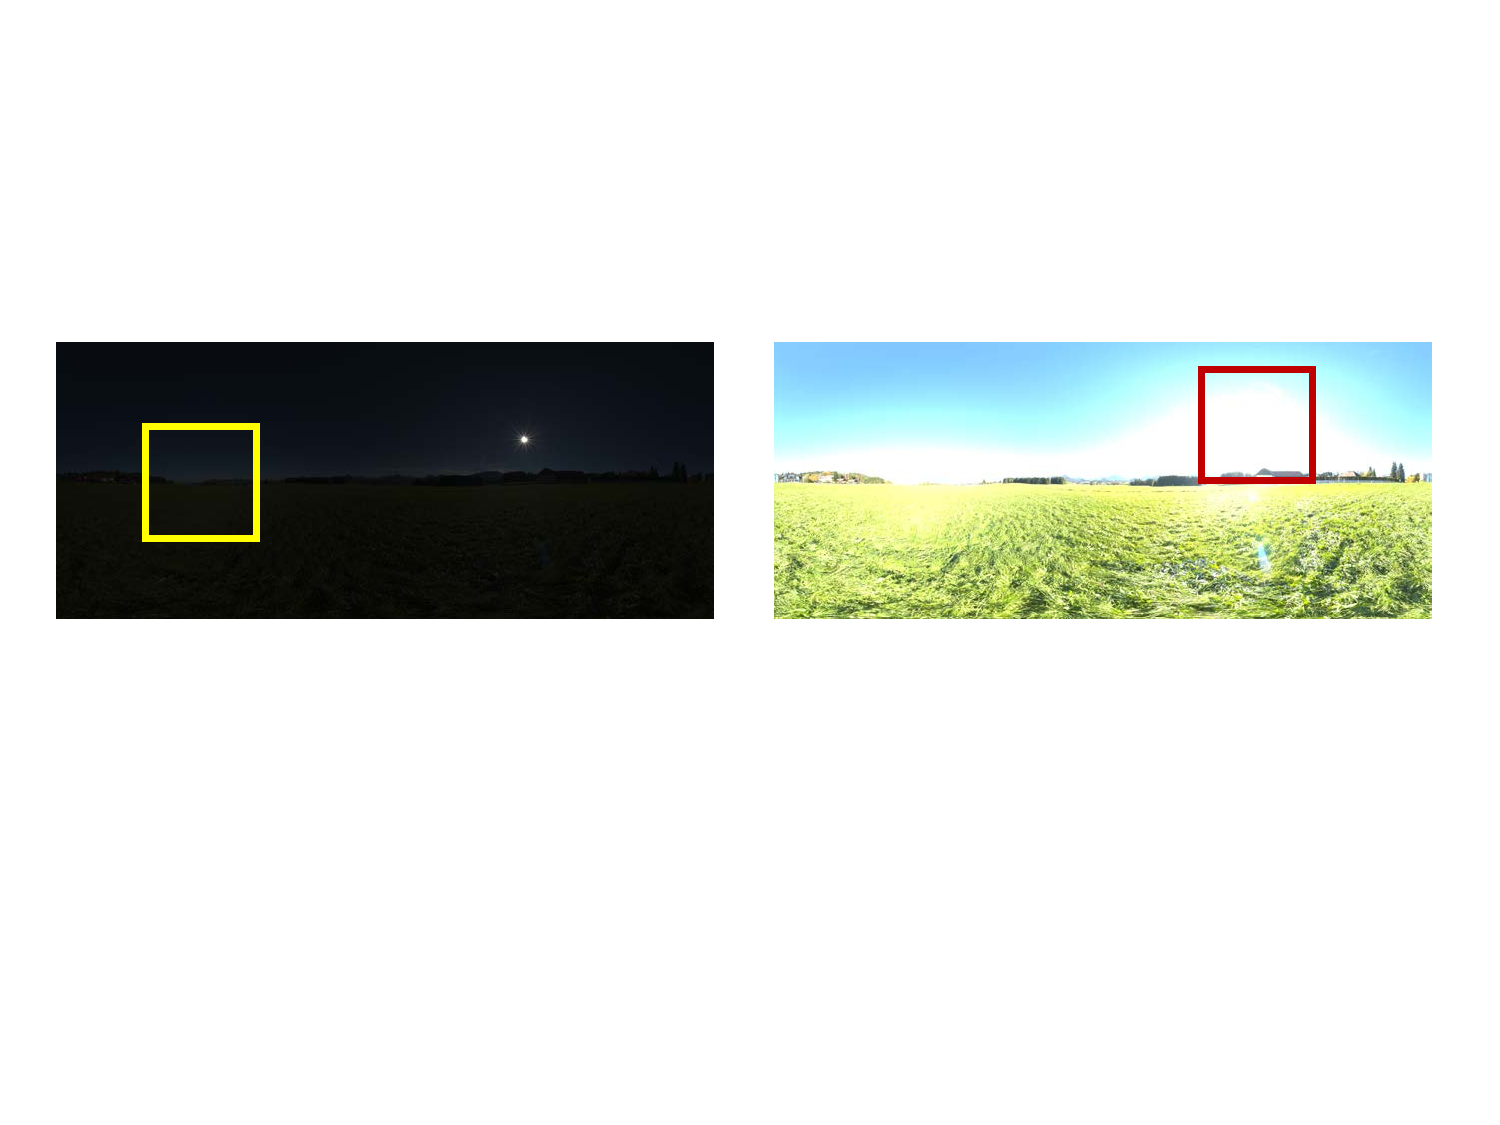
\includegraphics[width=1.0\textwidth]{Img/different-exposure.pdf}
    \caption[使用不同曝光拍摄的LDR图像]
    {两种不同曝光条件下的LDR图像。可以看出这两个图像都有过曝和欠曝的部分。在欠曝图像中,虽然黄色框选的区域中大部分像素均为黑色,但其实它们的明暗程度是不同的;类似地,在过曝图像中,虽然红色框选的区域中大部分像素均为白色,但实际上太阳所处像素的亮度是远远高于周围像素的。由于LDR图像动态范围较低,因此它无法作为真实光照的表示。}
    \label{fig:different-exposure}
\end{figure}